\documentclass[12pt]{article}
\usepackage{graphicx}
\usepackage{wrapfig}
\usepackage{subfigure}
\usepackage{multirow}
\usepackage{hyperref}
\usepackage{amsmath}
\usepackage{amssymb}
\usepackage{ngerman}
\usepackage[ansinew]{inputenc}
\usepackage[left=2cm,top=1cm]{geometry}

% vector graphics test
\usepackage{color}
\usepackage{transparent}
\graphicspath{{graphs/}}





\begin{document}
	\pagestyle{empty}
	\textasciitilde

\begin{titlepage}
    \centering
	\huge{Astronomisches Praktikum: Die Hubble-Konstante}\\
	\bigskip
    \large{Versuch 3}\\
    \huge{Jan R\"{o}der \& Julia Lienert}
\end{titlepage}

%headline!!!


\tableofcontents
\pagebreak

\section{Einleitung}

\section{Methoden zur Entfernungsbestimmung}
\subsection{Cepheidenmethode}
Cepheiden sind Sterne, die ihre Helligkeit periodisch �ndern. Durch Beobachtung der Periode kann �ber die Perioden-Leuchtkraft-Beziehung
\begin{equation}
	M = -2.81 \log\left(\frac{P}{\text{Tage}}\right) -1.43
\end{equation}
auf die absolute Helligkeit geschlossen werden. Zusammen mit der scheinbaren (beobachteten) Helligkeit l�sst sich der Abstand �ber das Entfernungsmodul berechnen.
\begin{equation}
	m - M = 5 \log\left(\frac{r}{10\,\text{pc}}\right)
\end{equation}
Diese Methode ist bis zu einigen Megaparsec anwendbar. Mit dem Hubble-Space-Telescope k�nnen sogar Sterne in bis zu $20 \,$pc Entfernung beobachtet und vermessen werden, was eine Beobachtung auch in benachbarten Galaxien m�glich macht.
 
\subsection{Parallaxenmethode}
Bei dieser Methode wird die scheinbare Bewegung naher Sterne vor einem Fixsternhintergrund weit entfernter Sterne gemessen. Sie kommt dadurch zustande, dass sich die Erde im Lauf eines Jahres um die Sonne bewegt.
\begin{figure} [h]
	\centering
	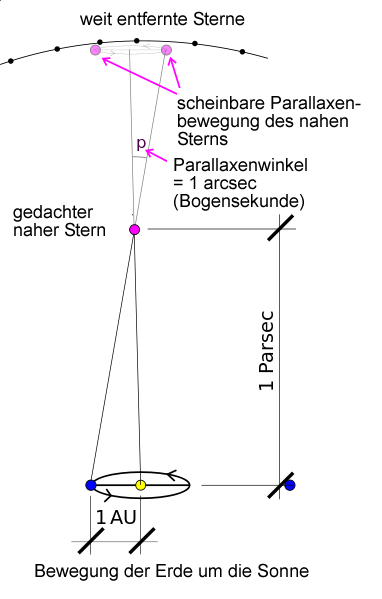
\includegraphics[width=0.5\textwidth]{Parallaxe.png}
	\caption{Skizze zur Erkl�rung der Parallaxe (entnommen aus [1])}
\end{figure}








\section{Quellen}
\begin{enumerate}
	\item $https://de.wikipedia.org/wiki/Parallaxe$
\end{enumerate}

\pagebreak



\begin{thebibliography}{2}
%\bibitem{Eichler} H. J. Eichler, H.-D. Kronfeldt, J. Sahm, \textit{Das Neue Physikalische Grundpraktikum}, Springer-Verlag, Berlin-Heidelberg, 2001.
%\bibitem{Kuchling} H. Kuchling, \textit{Taschenbuch der Physik, 21. Auflage}, Fachbuchverlag Leipzig, 2014.
\end{thebibliography}

\end{document}